\chapter{Bilder} \label{sec:pictures}

\section{Einzeln}

\begin{figure}[H]
    \begin{center} 
        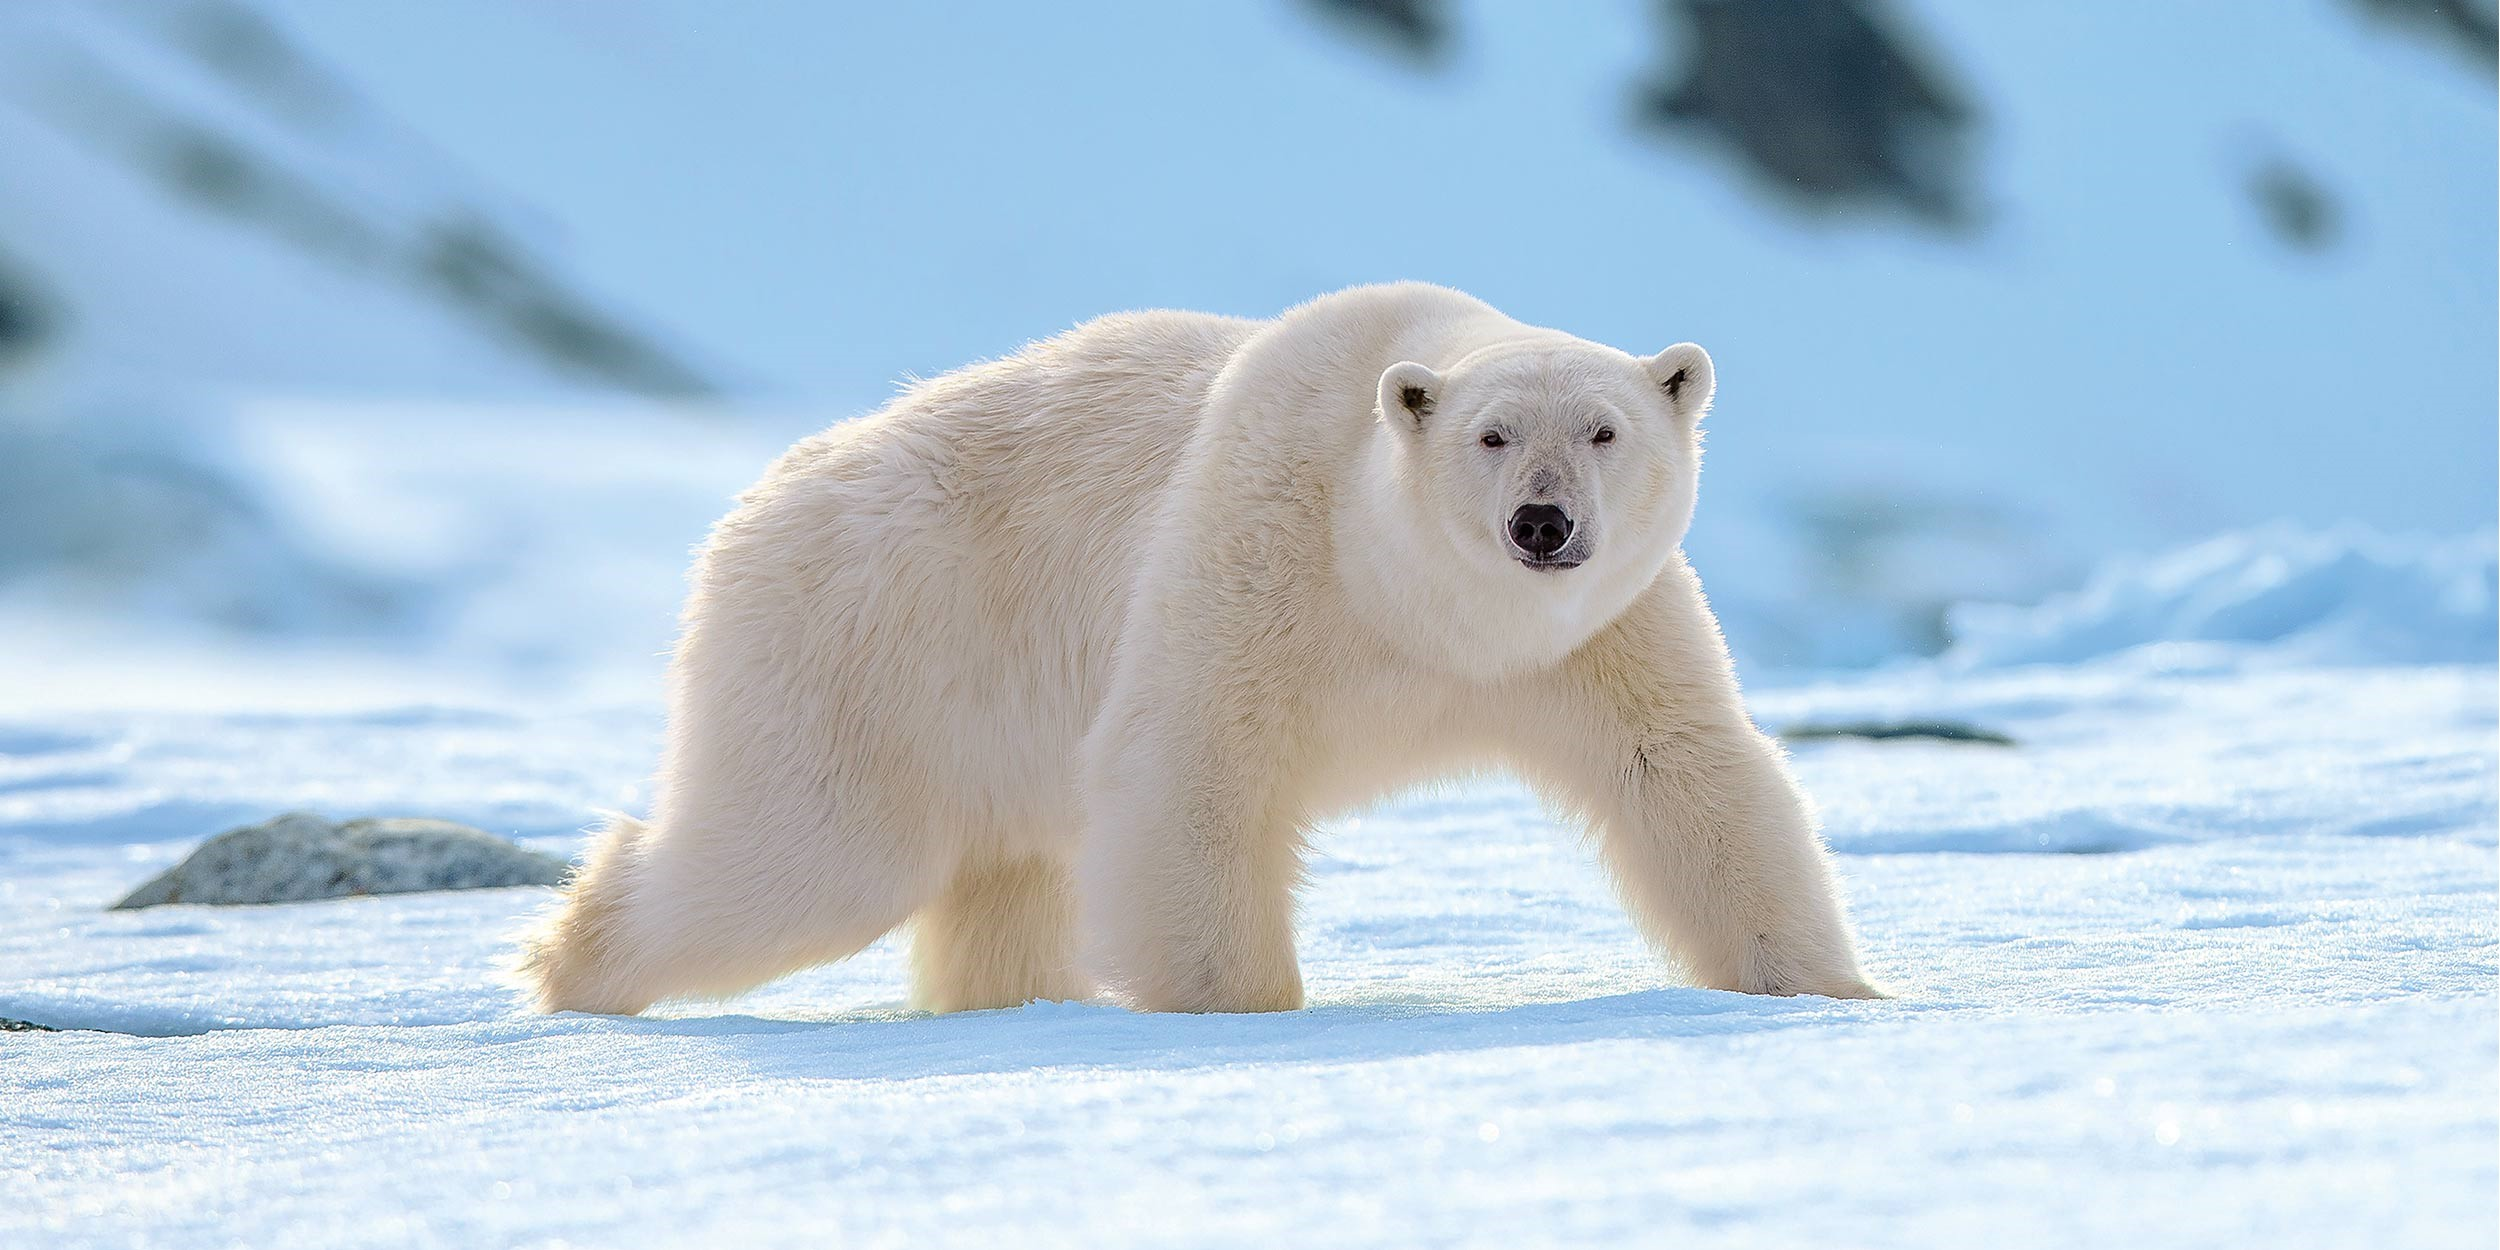
\includegraphics[width=0.5\linewidth]{example}
        \caption{Beispielbild 1}
        \label{fig:example-1}
    \end{center}
\end{figure}

\newpage

\section{Doppelt}

\begin{figure}[H]
    \begin{center} 
    \begin{subfigure}[b]{0.48\linewidth}
        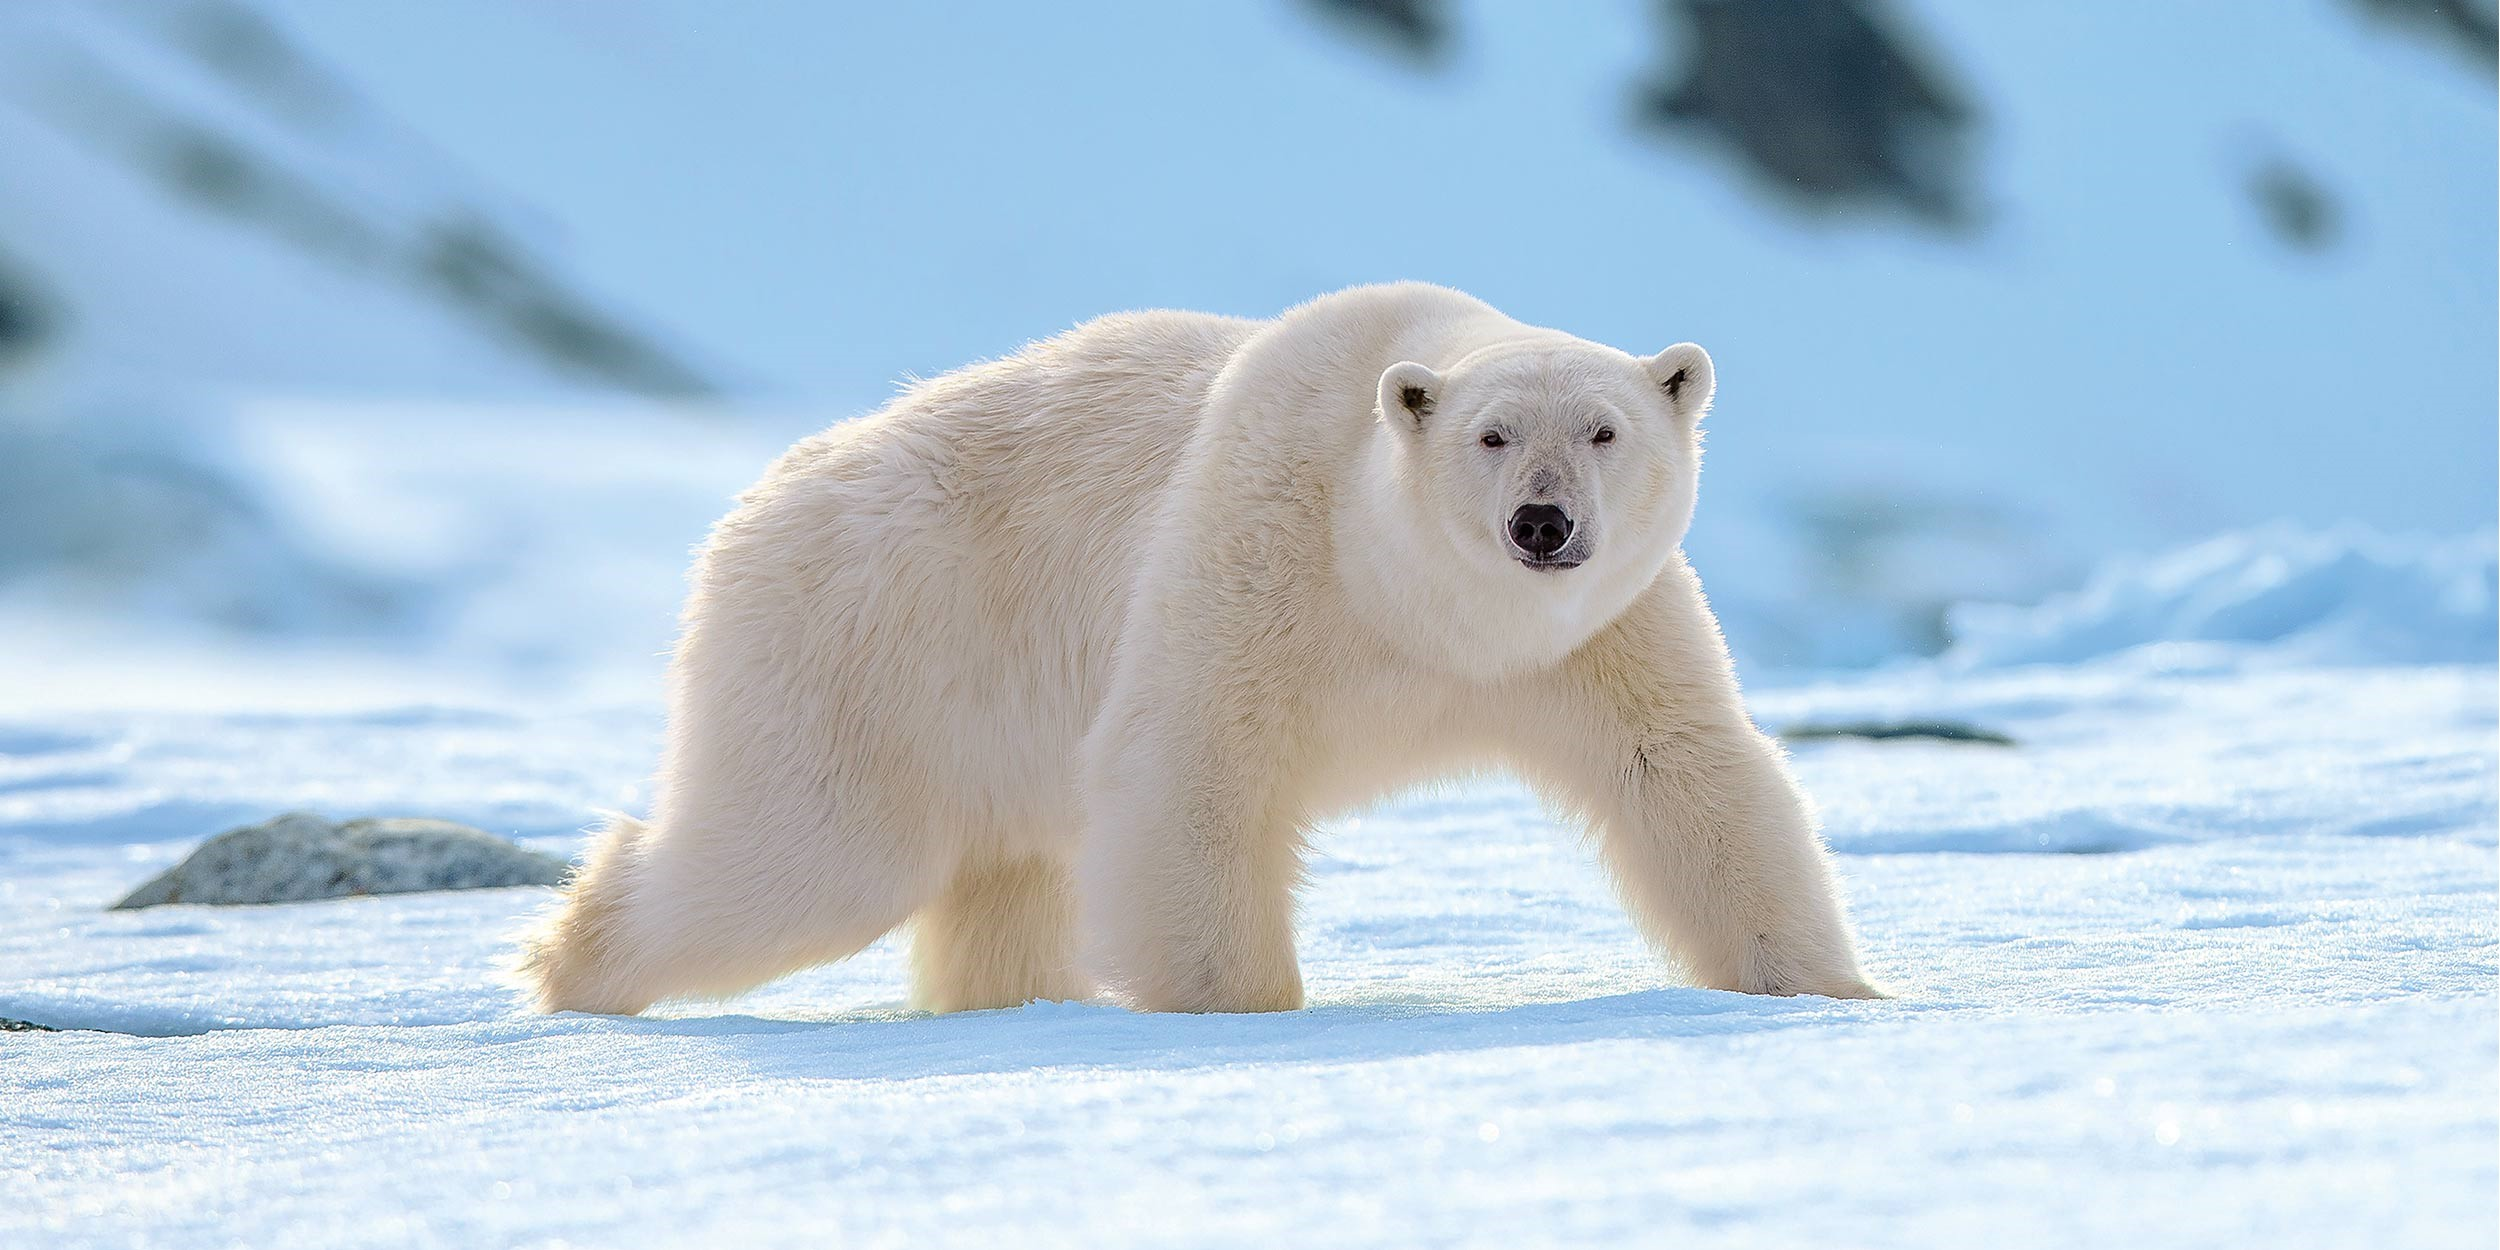
\includegraphics[width=\textwidth]{example}
        \caption{Beispielbild 2}
        \label{fig:example-2}
    \end{subfigure}
    \begin{subfigure}[b]{0.48\linewidth}
        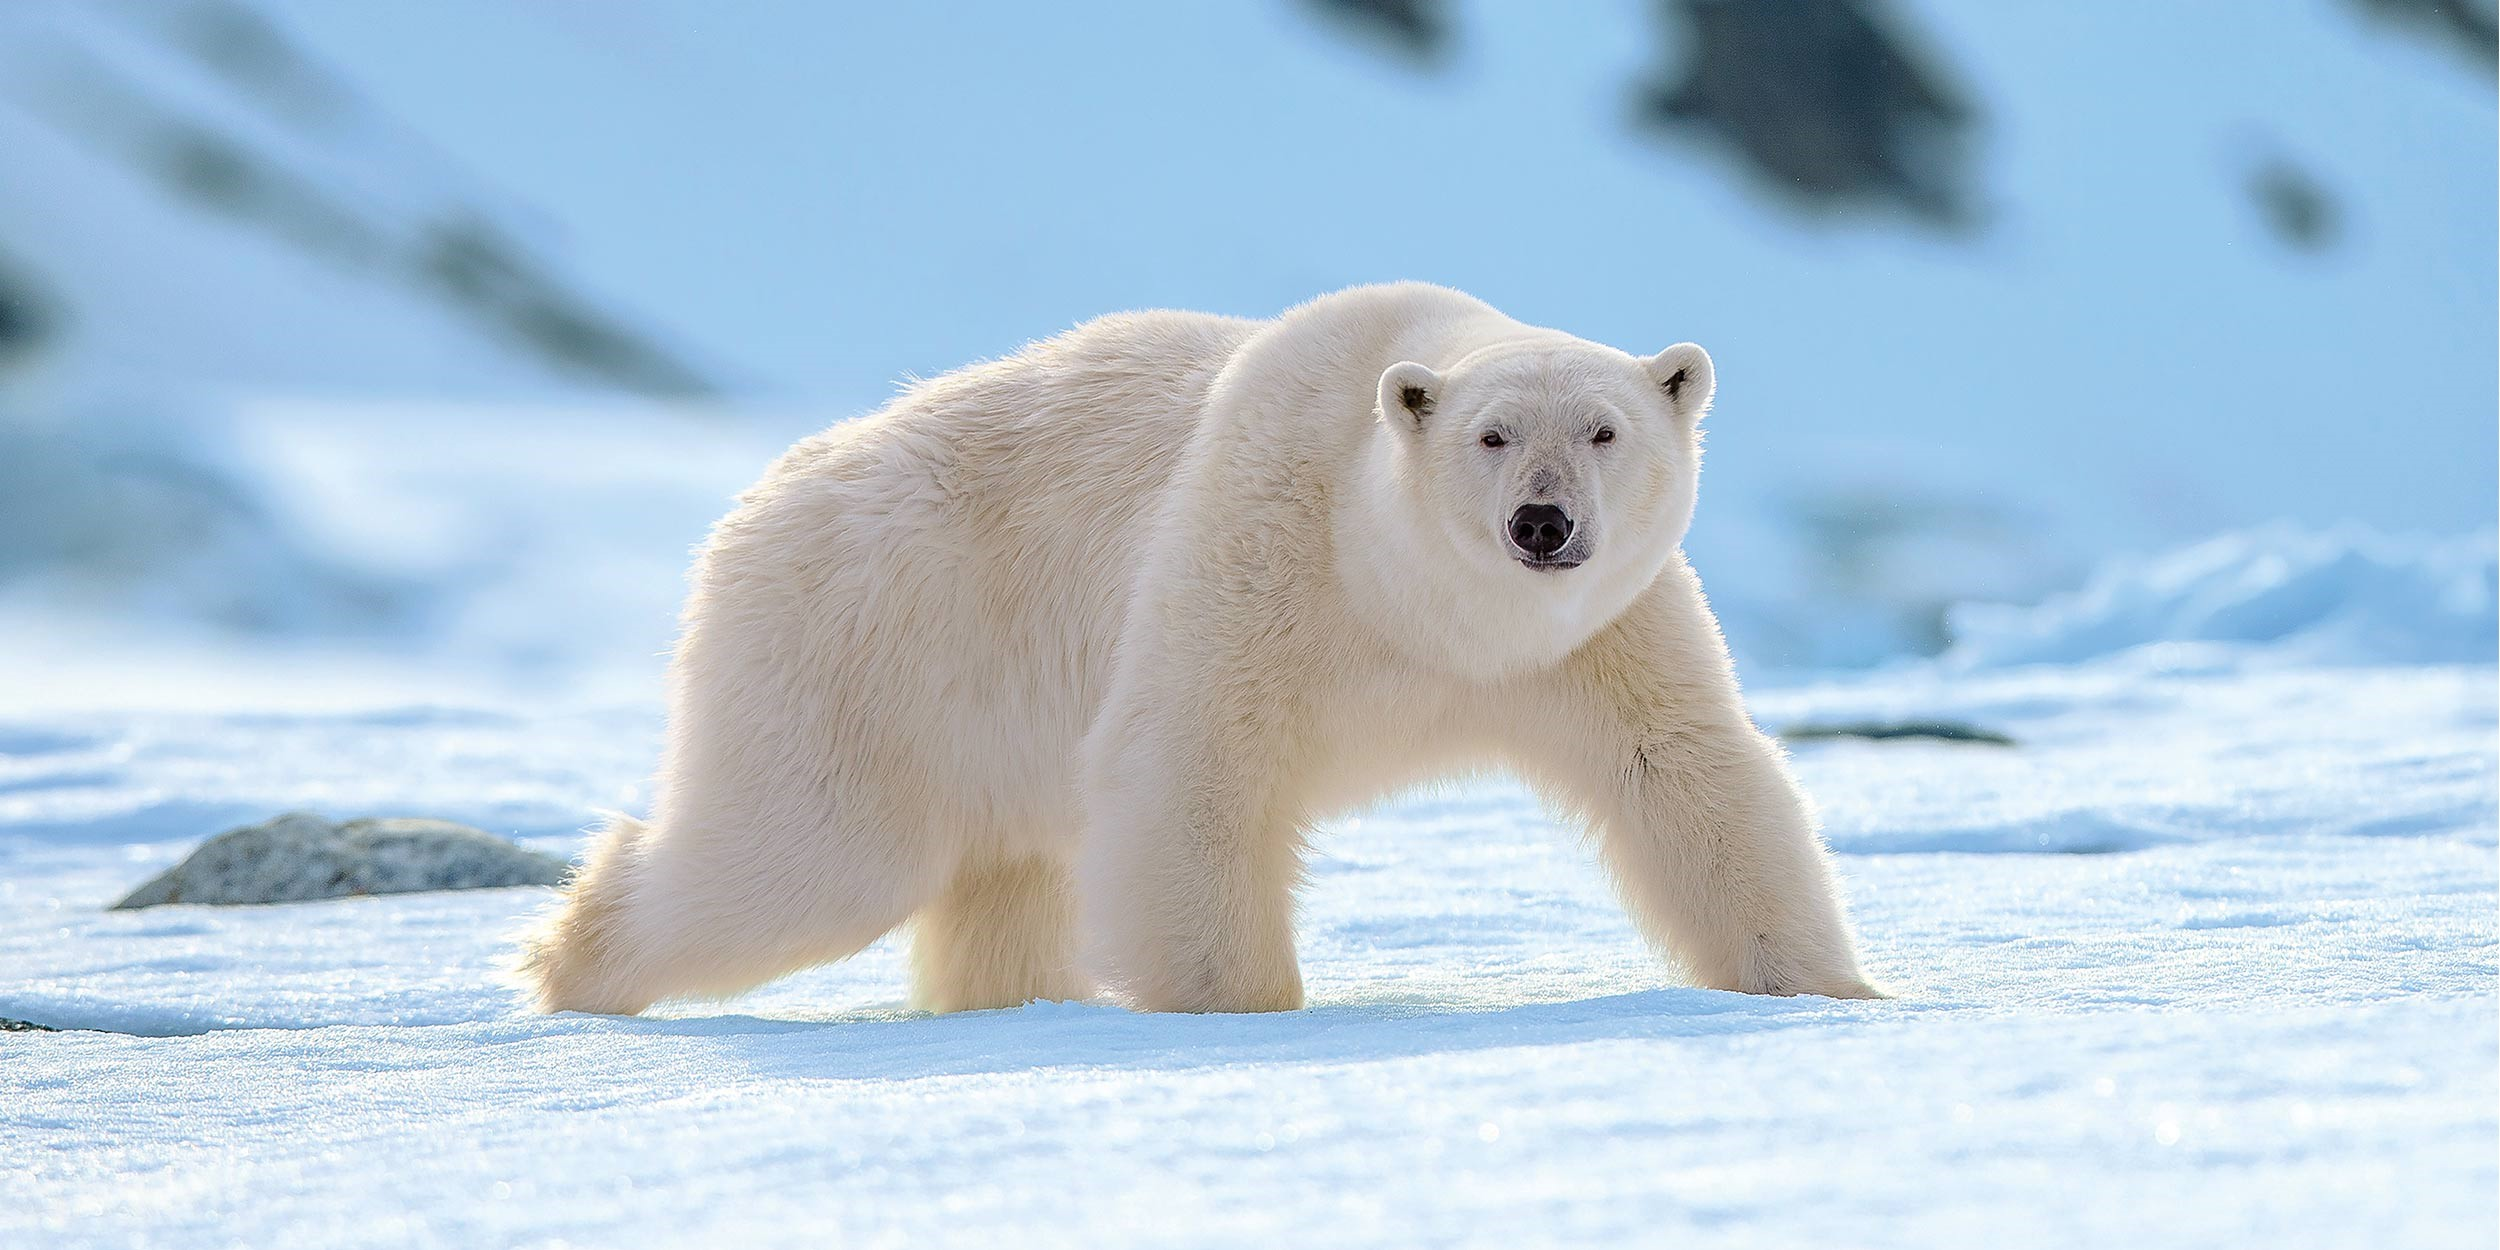
\includegraphics[width=\textwidth]{example}
        \caption{Beispielbild 3}
        \label{fig:example-3}
    \end{subfigure}
    \caption{Beispielbilder}
    \label{fig:examples}
    \end{center}
\end{figure}

Die \refa{fig:example-2} ist super!

Schau dir mal \refk{sec:pictures} an!

\chapter{Bibliography}

\cite[vgl.][]{example-book}

\cite[][ein Bild]{example-online}

Vielleicht reicht auch Google\wwwlink{google.de}...

\chapter{Abkürzungen}

\ac{html} ist super. \acf{js} wird ausgeschrieben \engl{written out}. \acs{js} wird nur abgekürzt.

\chapter{Programmierung}

\section{Lstlisting}

\begin{lstlisting} [caption=Zugriff auf Klassen über eine Nachschlagetabelle, label=code:lookup-table]
    const bgColor = {
        blue: "bg-blue-600",
        red: "bg-red-600",
        green: "bg-green-600",
    };
    bgColor[props.color]
\end{lstlisting}

\section{Verbatim}

\begin{verbatim}
$ sudo apt-get update
$ sudo apt-get install python
\end{verbatim}

\chapter{Glossary}

\gls{glos:latex}

\gls{glos:swagger}
